\chapter{Membangun Model Prediksi}

Your related works, and your purpose and contribution which must be different as below.

\section{Fadila/1164072}
\subsection{Teori}
Penyelesaian Tugas Harian 3 ( No. 1-7 )
\begin{enumerate}
\item Binary Classification Dan Ilustrasi Gambarnya
\begin{itemize}
\item Pengertian Binary Classification / Klasifikasi Biner:
\par Klasifikasi biner atau binomial merupakan tugas untuk mengklasifikasikan elemen-elemen dari himpunan tertentu ke dalam dua kelompok (memprediksi kelompok mana yang masing-masing dimiliki) ber-
\par dasarkan aturan klasifikasi.
\item Ilustrasi Gambar Binary Classification :
\par

\begin{figure}[ht]
\centering
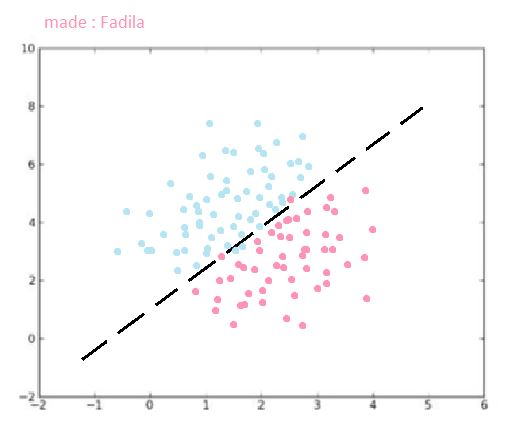
\includegraphics[scale=0.3]{figures/binary.jpg}
\caption{binary classification}
\label{contoh}
\end{figure}

\par
\end{itemize}
\item Supervised Learning, Unsupervised Learning, Clustering Dan Ilustrasi Gambar
\begin{itemize}
\item Pengertian Supervised Learning :
\par Sebuah pendekatan dimana terdapat data yang dilatih dan ditargetkan. Leih singkatnya supervised learning memiliki kategori sehingga tujuan dan outputnya jelas.
\begin{itemize}
\par
\item Ilustrasi Gambar Supervised Learning :

\begin{figure}[ht]
\centering
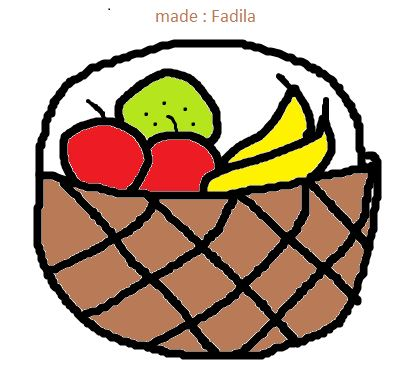
\includegraphics[scale=0.4]{figures/supervised1.jpg}
\caption{supervised}
\label{contoh}
\end{figure}


\par Pada contoh gambar diatas dikelompokkan bahwa apabila bentuk dari objek di gambar berbentuk bundar dan berwarna merah maka akan dinamakan atau di sebut sebagai Apel. Dan apabila pada gambar terdapat objek berbentuk panjang dan berwarna kuning maka akan dinamakan atau di sebut sebagai pisang.
\par
\end{itemize}

\par
\item Pengertian Unsupervised Learning :
\par Tidak memiliki data latih, sehingga dari data yang tersebut kita bisa mengelompokkannya ke berbagai kelompok 2 seterusnya. Dengan lebih singkatnya ialah unsupervised learning tidak memiliki kategori.
\par
\par
\begin{itemize}
\item Ilustrasi Gambar Unsupervised Learning :

\begin{figure}[ht]
\centering
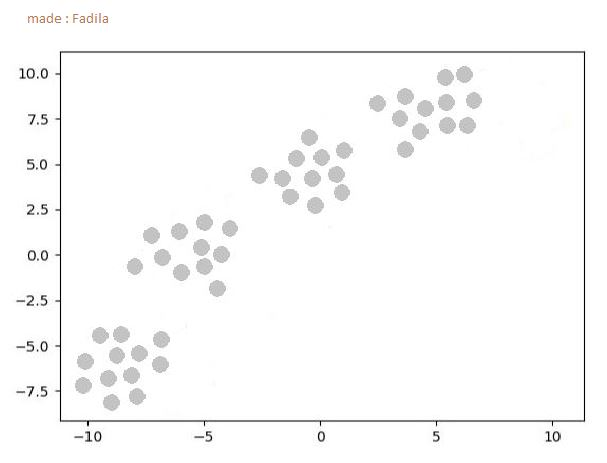
\includegraphics[scale=0.4]{figures/unsupervised2.jpg}
\caption{unsupervised}
\label{contoh}
\end{figure}

\par Pada gambar dapat dilihat bahwa ada banyak data namun tidak pada pengelompokkan yang tepat. Cuman dapat dikelompokkan ke dalam berbagai macam bentuk dan jumlah namun tidak memberikan output yang jelas.
\par
\par
\end{itemize}
\item Pengertian Clustering :
\par Metode pengelompokan data. Clustering juga merupakan proses partisi satu set objek data ke dalam himpunan bagian yang disebut dengan cluster. Objek dalam cluster tersebut memiliki kemiripan karakteristik antar satu sama lain.
\par

\begin{figure}[ht]
\centering
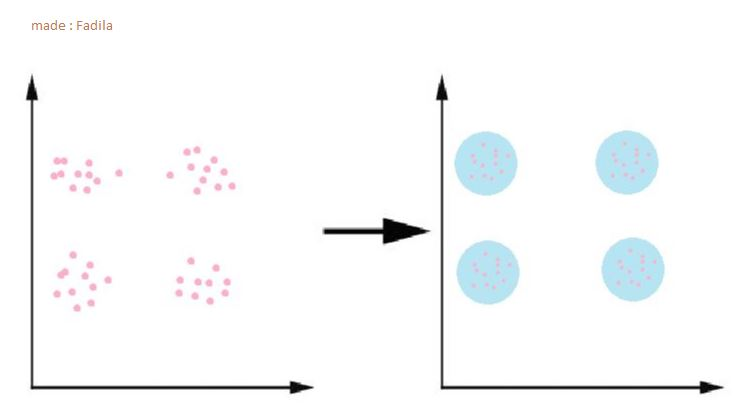
\includegraphics[scale=0.5]{figures/clustering.jpg}
\caption{clustering}
\label{contoh}
\end{figure}

\par
\end{itemize}
\item Evaluasi, Akurasi Dan Ilustrasi Gambar
\begin{itemize}
\item Pengertian Evaluasi
\par Evaluasi digunakan untuk memeriksa/memastikan dan mengevaluasi model dalam bekerja ( seberapa baik ) dengan mengukur keakuratannya. Kita juga dapat menanalisis kesalahan yang dibuat pada model yang dijalankan, tingkat kebingungan dan menggunakan matriks kebingunan.
\begin{figure}[ht]
\centering
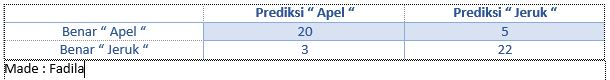
\includegraphics[scale=0.6]{figures/eva.jpg}
\caption{Evaluasi}
\label{contoh}
\end{figure}

\par Pada contoh gambar dapat dilihat bahwa dilakukan evaluasi terhadap kerja dalam penentuan jenis dari objek. Dievaluasi berapa banyak sebuah objek ketika dikelompokkan dan diklasifikasikan kemudian dapat dilihat apakah kerjanya sesuai atau tidak.
\par

\par
\item Pengertian Akurasi
\par Accuracy akan didefinisikan sebagai presentasi kasus yang diklasifikasikan dengan benar. Accuracy lebih jelasnya adalah perbandingan kasus yang diidentifikasi benar dengan jumlah semua kasus
\par Rumus dari accuracy= (a+c)/(a+b+c+d)
\par

\begin{figure}[ht]
\centering
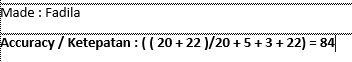
\includegraphics[scale=0.8]{figures/acuracy.jpg}
\caption{Akurasi}
\label{contoh}
\end{figure}

\par Dilakukan perhitungan dengan rumus akurasi terhadap data yang telah diolah pada " Evaluasi ". Kemudian di dapatkan hasil dari pengolahan data tersebut.
\par Contoh penggabungan Akurasi Dan Evaluasi
\par

\begin{figure}[ht]
\centering
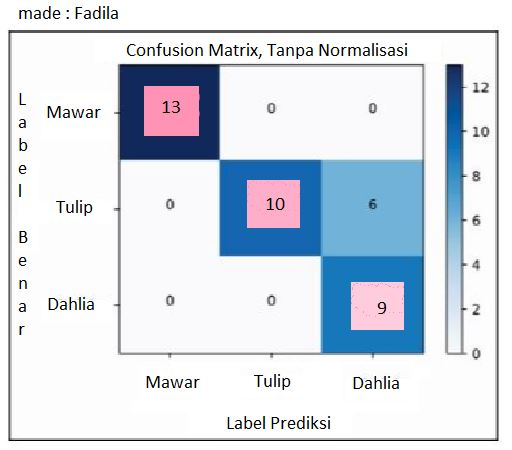
\includegraphics[scale=0.5]{figures/evacuray.jpg}
\caption{Contoh Evaluasi Dan Akurasi Secara Bersamaan }
\label{contoh}
\end{figure}

\end{itemize}

\par
\item Membuat Dan Membaca Confusion Matrix Beserta Contoh
\begin{itemize}
\item Pengertian Confusion Matrix
\par Confusion matrix merupakan suatu metode yang digunakan untuk melakukan perhitungan akurasi pada konsep data mining.
\item Pembacaan Confusion Matrix
\begin{enumerate}
\item Apabila hasil prediksi negatif dan data sebenarnya merupakan negatif.
\item Apabila hasil prediksi positif sedangkan nilai sebenarnya merupakan negatif.
\item Apabila hasil prediksi negatif sedangkan nilai sebenarnya merupakan positif.
\item Apabila hasil prediksi positif dan nilai sebenarnya merupakan positif.
\end{enumerate}
\par
\par
\item Pembuatan Confusion Matrix
\begin{enumerate}
\item Menentukan 4 proses klasifikasi yang akan digunakan dalam confusion matrix.
\item 4 Istilah tersebut ada True Positive ( TP ), True Negative ( TN ), False Positive ( FP ) dan False Negative ( FN ).
\item Kelompokkan klasifikasi tersebut bisa menggunakan klasifikasi biner
\item Akan menghasilkan keluaran berupa 2 Kelas ( Positif dan Negatif ) dan penentuan TP, FP ( 1 klasifikasi positif ) , FN dan TN ( 1 klasifikasi negatif ).
\item Contoh dasarnya nampak seperti langkah diatas
\item Istilahnya daat didefinisikan dengan objek lain namu dengan alur yang sama ( sesuai rumus baik klasifikasi dll ).
\end{enumerate}
\par

\item Ilustrasi Gambar
\par

\begin{figure}[ht]
\centering
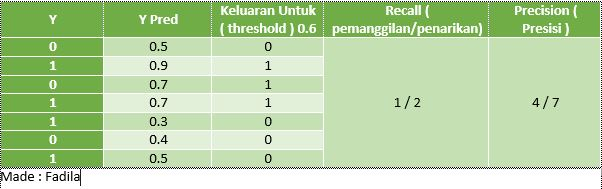
\includegraphics[scale=0.6]{figures/confusion.jpg}
\caption{confusion matrix}
\label{contoh}
\end{figure}

\par
\begin{itemize}
\item Penjelasan
\begin{enumerate}
\item Recall
\par Dari semua kelas positif, seberapa banyak yang kami prediksi dengan benar. Itu harus setinggi mungkin.
\par

\begin{figure}[ht]
\centering
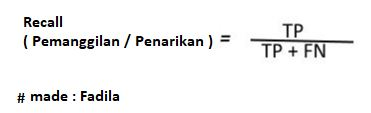
\includegraphics[scale=0.6]{figures/recall.jpg}
\caption{recall}
\label{contoh}
\end{figure}

\par
\item Presisi / Precision
\par Dari semua kelas, seberapa banyak yang kami prediksi dengan benar. Itu harus setinggi mungkin.
\par

\begin{figure}[ht]
\centering
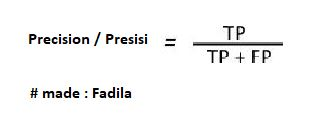
\includegraphics[scale=0.6]{figures/precision.jpg}
\caption{precision}
\label{contoh}
\end{figure}

\par
\item F-Ukur ( measure )
\par Sulit untuk membandingkan dua model dengan presisi rendah dan daya ingat tinggi atau sebaliknya. Jadi untuk membuatnya sebanding, kami menggunakan F-Score. F-score membantu mengukur Recall dan Precision pada saat yang bersamaan
\par

\begin{figure}[ht]
\centering
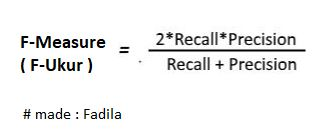
\includegraphics[scale=0.6]{figures/f.jpg}
\caption{f-measure}
\label{contoh}
\end{figure}

\par
\end{enumerate}
\end{itemize}
\end{itemize}


\par
\item Cara Kerja K-Fold Classification Dan Ilustrasi Gambar
\begin{enumerate}
\item Pertama-tama untuk total instance dibagi menjadi N bagian.
\item Fold ke-1 ( atau pertama ) adalah ketika bagian ke-1 menjadi data uji (testing data) dan sisanya menjadi data latih (training data).
\item Hitung akurasi ( berdasarkan porsi data tersebut. Persamaanya sebagai berikut :
\par (sigma) data klasifikasi
\par (sigma) total data uji
\par x 100 persen 
\item Fold ke-2 ( kedua ) adalah ketika bagian ke-2 menjadi data uji (testing data) dan sisanya menjadi data latih (training data). 
\item Kemudian dihitunglah akurasi berdasarkan porsi data yang telah ditentukan
\item Demikian seterusnya hingga mencapai fold ke-K. Hitung rata-rata akurasi dari K buah akurasi di atas. Rata-rata akurasi ini menjadi akurasi final atau akhir.
\end{enumerate}
\par
\begin{itemize}
\item Ilustrasi Gambar
\par

\begin{figure}[ht]
\centering
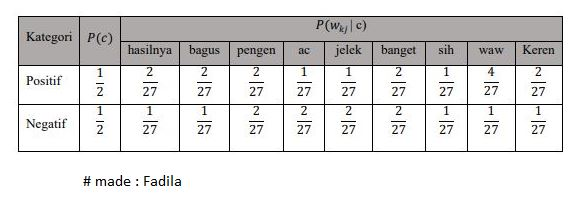
\includegraphics[scale=0.4]{figures/hasilk1.jpg}
\caption{k-fold classification 1}
\label{contoh}
\end{figure}

\begin{figure}[ht]
\centering
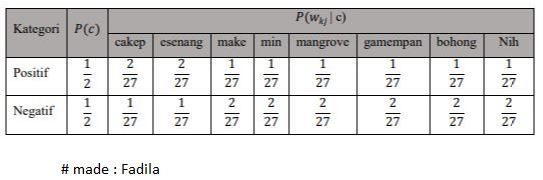
\includegraphics[scale=0.4]{figures/hasilk2.jpg}
\caption{k-fold classification 2}
\label{contoh}
\end{figure}

\par
\par
\end{itemize}

\par
\item Decision Tree Dan Ilustrasi Gambar
\begin{itemize}
\item Pengertian Decision Tree
\par Decision tree adalah salah satu metode klasifikasi yang paling populer karena mudah diinterpretasikan oleh manusia. Decision tree merupakan metode klasifikasi yang digunakan untuk pengenalan pola dan termasuk dalam pengenalan pola secara statistik. 3 tipe dari decision tree ialah: simpul: simpul root, simpul perantara, dan simpul leaf.
\par

\end{itemize}
\par

\par
\begin{itemize}
\item Ilustrasi Gambar
\par


\begin{figure}[ht]
\centering
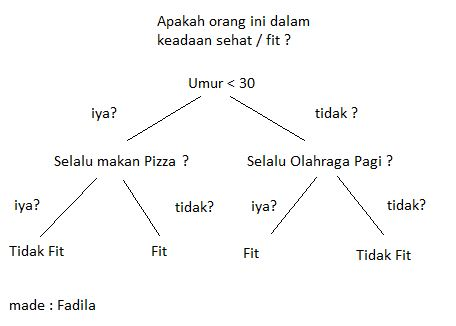
\includegraphics[scale=0.5]{figures/decisiontree.jpg}
\caption{decision tree}
\label{contoh}
\end{figure}

\par
\end{itemize}
\item Information Gain Dan Entropi
\begin{itemize}
\item Pengertian Information Gain
\par Information Gain adalah salah satu atribute selection measure yang digunakan untuk memilih test atribute tiap node pada tree.
\par Algoritme Information Gain digunakan untuk mengurangi dimensi atribut untuk mendapatkan atribut-atribut yang relevan. 
\par

\begin{itemize}
\item Ilustrasi Gambar
\par


\begin{figure}[ht]
\centering
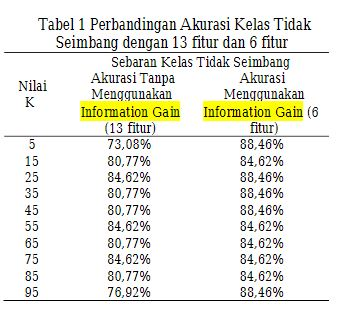
\includegraphics[scale=0.6]{figures/information1.jpg}
\caption{informaion gain 1}
\label{contoh}
\end{figure}


\begin{figure}[ht]
\centering
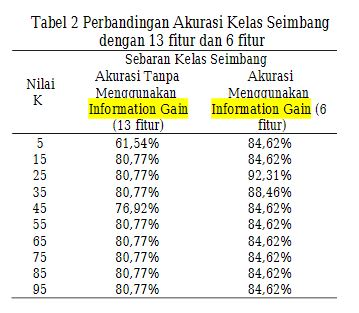
\includegraphics[scale=0.6]{figures/information2.jpg}
\caption{information gain 2}
\label{contoh}
\end{figure}

\item Penjelasan :
\par Tabel 1 sampai dengan Tabel 2 menunjukkan bahwa penggunaan seleksi fitur Information Gain menghasilkan nilai akurasi yang lebih baik dibandingkan tanpa menggunakan Information Gain. 
\par Pada saat nilai K sama dengan 5 ( K=5) akurasi yang dihasilkan sistem tanpa menggunakan Information Gain menunjukkan hasil yang kurang baik pada sebaran kelas seimbang maupun tak seimbang yaitu 61,54 persen pada sebaran kelas seimbang dan 73,08 persen pada sebaran kelas tidak seimbang. 
\end{itemize}


\par
\item Pengertian Entropi
\par Entropi pada umumnya merupakan salah satu besaran yang mengukur energi dalam sistem per satuan temperatur yang tak dapat digunakan untuk melakukan usaha.
\par Namun, secara spesifik untuk " Entropi " sendiri merupakan parameter untuk mengukur tingkat keberagaman (heterogenitas) dari kumpulan data. 

\par

\begin{figure}[ht]
\centering
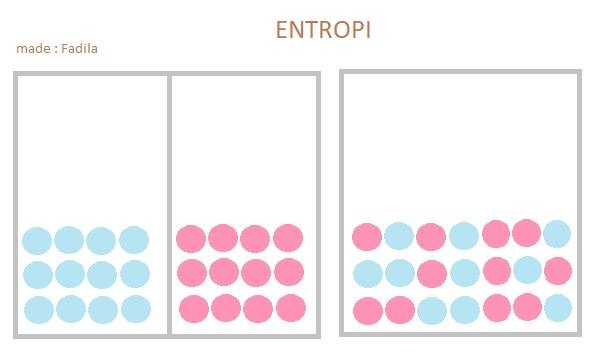
\includegraphics[scale=0.5]{figures/entropi.jpg}
\caption{entropi}
\label{contoh}
\end{figure}

\par
\end{itemize}

\subsection{Praktek Scikit-Learn}
Penyelesaian Tugas Harian 4 ( No. 1-12 )
\begin{enumerate}
\item Pembahasan Codingan Dan Hasilnya
\begin{enumerate}
\item Codingan Pertama :
\par Penjelasan : Codingan pertama ini akan meload ( menampilkan ) data pada file yang ditentukan. Untuk codingan ini file yang dieksekusi ialah " student-mat.csv " . Secara jelasnya, dalam codingan dapat dilihat bahwa variabel bakso didefinisikan untuk pembacaan csv dari " pizza " dimana untuk pemisahnya yaitu separation berupa ; . Setelah itu variabel bakso di "print" dengan perintah menampilkan "len" panjang ataupun jumlah dan hasilnya berupa angka 395 . 
\par
\begin{itemize}
\par
\item Hasil Codingan Pertama :
\par

\begin{figure}[ht]
\centering
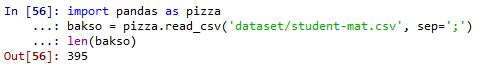
\includegraphics[scale=0.7]{figures/hasil1.jpg}
\caption{codingan pertama}
\label{contoh}
\end{figure}

\par
\end{itemize}
\item Codingan Kedua :
\par Penjelasan : Codingan kedua ini secara keseluruhan menampilkan  baris  G1, G2 dan G3 ( berdasarkan kriterianya ) untuk kolom PASS pada variabel bakso. Untuk lebih jelasnya, pada codingan terdapat pendefinisian pembacaan "lamda" ( panjang gelombang ) dari baris G1, G2 dan G3. Apabila row-row tersebut bernilai lebih dari 35 maka akan terdefinisikan angka "1" apabila tidak, maka akan terdefinisikan angka "0" pada kolom PASS ( sesuai permintaan awal ). Selanjutnya variabelnya di "print" sehingga menampilkan keluaran. Tidak lupa terdapat juga jumlah dari baris dan kolom yang terubah sesuai dengan baris yang dieksekusi.
\par 
\begin{itemize}
\par
\item Hasil Codingan Kedua :

\begin{figure}[ht]
\centering
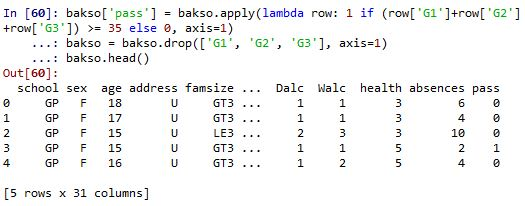
\includegraphics[scale=0.7]{figures/hasil2.jpg}
\caption{codingan kedua}
\label{contoh}
\end{figure}

\end{itemize}
\par
\item Codingan Ketiga :
\par Penjelasan : Secara keseluruhan, codingan ini mendefinisikan pemanggilan get dummies dari pizza dalam variabel bakso. Di dalam get dummies sendiri akan terdefinisikan variabel bakso dengan kolom-kolom yang akan dieksekusi seperti school, address dll. Kemudian variabel tersebut di definisikan untuk mendapatkan kembalian berupa keluaran dari eksekusi perintah variabel bakso beserta dengan jumlah baris dan kolom data yang dieksekusi.
\par 
\begin{itemize}
\par
\item Hasil Codingan Ketiga :

\begin{figure}[ht]
\centering
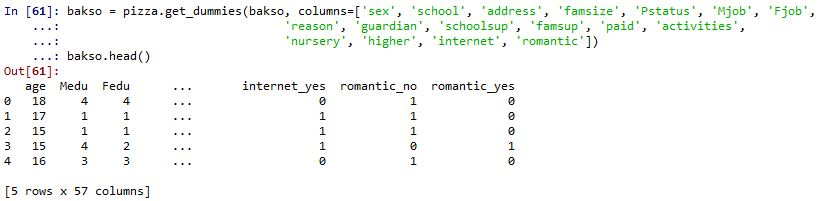
\includegraphics[scale=0.4]{figures/hasil3.jpg}
\caption{codingan ketiga}
\label{contoh}
\end{figure}

\end{itemize}
\par
\item Codingan Keempat :
\par Penjelasan : Secara keseluruhan codingan ini difungsikan untuk mendefinisikan pembagian data yang berupa training dan testing data. Secara jelasnya pertama-tama variabel bakso akan mendefinisikan sampel yang akan digunakan ( berupa shuffle row ) . Nah kemudian masing2 parameter yaitu bakso train dan bakso test akan berjumlah 500 data ( telah dibagi untuk training dan testing ). Selanjutnya dilakukan pengeksekusian untuk kolom Pass, apabila sesuai dengan "axis=1" maka eksekusi fungsi berhasil. Selain itu juga disertakan jumlah dari peserta yang lolos dari semua nilai data setnya.  
\par 
\begin{itemize}
\par
\item Hasil Codingan Keempat :

\begin{figure}[ht]
\centering
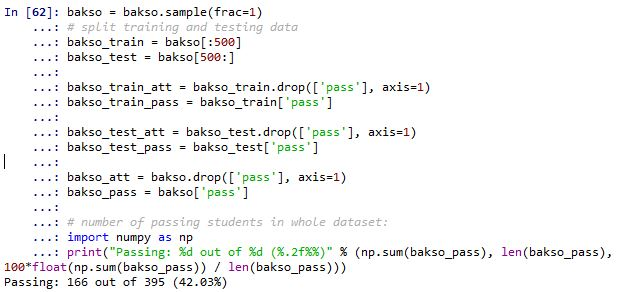
\includegraphics[scale=0.4]{figures/hasil4.jpg}
\caption{codingan keempat}
\label{contoh}
\end{figure}

\end{itemize}
\par
\item Codingan Kelima :
\par Penjelasan : Secara keseluruhan, codingan ini hanya membuktikan pengujian dari Klasifikasi Decision Tree yang ada, apakah true atau tidak dan hasilnya true. Apabila dibahas secara lengkap maka pada codingan ini di definisikan library sklearn untuk mengimpor atau menampilkan tree. Variabel sate difungsikan untuk membaca klasifikasi decision tree dari tree itu sendiri dengan 2 parameternya yaitu kriteria="entropy" dan max depth=5. Maka selanjutnya variabel sate akan masuk dan terbaca dalam module fit dengan 2 parameter yaitu bakso trai att dan bakso train pass.
\par 
\begin{itemize}
\par
\item Hasil Codingan Kelima :

\begin{figure}[ht]
\centering
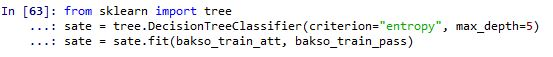
\includegraphics[scale=0.4]{figures/hasil5.jpg}
\caption{codingan kelima}
\label{contoh}
\end{figure}

\end{itemize}
\par
\item Codingan Keenam :
\par Penjelasan :  Codingan ini memberikan gambaran dari klasifikasi decision tree dari pengolahan parameter yang dieksekusi kedalam variabel sate. Tentunya dengan pemanfaatan library graphviz yang telah diimport dan difungsikan.
\par Untuk gambarnya terlalu besar ketika di Console sehingga hanya sebagian yang bisa di screenshoot untuk dijadikan hasil.
\begin{itemize}
\par
\item Hasil Codingan Keenam :

\begin{figure}[ht]
\centering
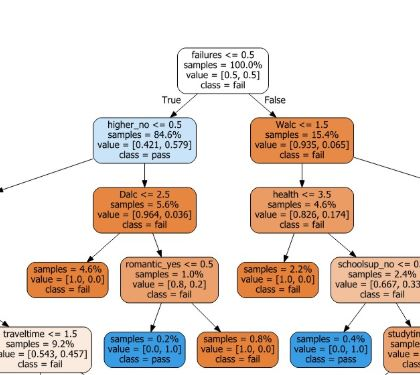
\includegraphics[scale=0.4]{figures/hasil6.jpg}
\caption{codingan keenam}
\label{contoh}
\end{figure}

\end{itemize}
\par
\item Codingan Ketujuh :
\par Penjelasan : Secara keseluruhan, codingan ini membahas tentang penyimpanan tree dari library graphiz yang dieksekusi bersamaan dengan variabel sate dan parameter lainnya. Dilakukan pengecekan dan pengujian apakah klasifikasi decision treenya dapat berjalan atau tidak. Apabila tidak berjalan, maka akan terjadi error, namun codingan ini berfungsi.
\par 
\begin{itemize}
\par
\item Hasil Codingan Ketujuh :

\begin{figure}[ht]
\centering
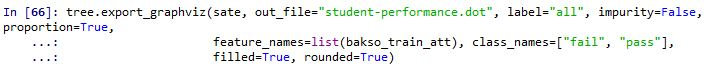
\includegraphics[scale=0.6]{figures/hasil7.jpg}
\caption{codingan ketujuh}
\label{contoh}
\end{figure}

\end{itemize}
\par
\item Codingan Kedelapan :
\par Penjelasan : Secara keseluruhan, codingan ini membaca score dari variabel sate dimana terdapat 2 parameter yang dihitung dan diuji yaitu bakso test att dan bakso test pass. Untuk hasilnya sendiri mengapa berupa angka, dikarenakan pada parameter yang dieksekusi memang memiliki data sehingga dieksekusi dan menghasilkan keluaran dari score tersebut.
\par 
\begin{itemize}
\par
\item Hasil Codingan Kedelapan :

\begin{figure}[ht]
\centering
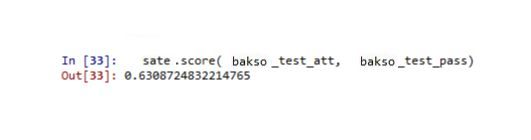
\includegraphics[scale=0.8]{figures/hasil8.jpg}
\caption{codingan kedelapan}
\label{contoh}
\end{figure}

\end{itemize}
\par
\item Codingan Kesembilan :
\par Penjelasan : Secara keseluruhan, codingan ini membahas mengenai pengkesekusian fungsi dan variabel dari library yang didefinisikan dan yang diimport. Penjelasan lebih jelasnya ialah codingan ini mendefinisikan library sklearn.model.selection kemudian mengimpor cross val score. Kemudian variabel score mendefinisikan cross val score yang telah diimport tadi dengan 4 parameter yaitu sate, bakso att, bakso pass dan cv=5 untuk dieksekusi. Setelah semua pemrosesan tersebut maka hasil yang di "print" ialah rata2 perhitungan dari variabel score dimana dan standar dari (+/-) tentunya dengan ketentuan parameter Accuracy .
\par 
\begin{itemize}
\par
\item Hasil Codingan Kesembilan :

\begin{figure}[ht]
\centering
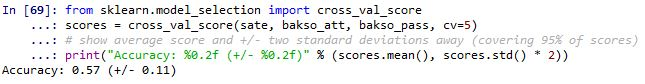
\includegraphics[scale=0.7]{figures/hasil9.jpg}
\caption{codingan kesembilan}
\label{contoh}
\end{figure}

\end{itemize}
\par
\item Codingan Ke-10 :
\par Penjelasan : Codingan ini mendefinisikan max depth dalam jarak angka antara parameter 1 dan 20. Variabel sate mendefinisikan klasifier decision tree dengan 2 parameter. Kemudian variabel score mengeksekusi parameter lainnya yaitu seperti sate, bakso att, bakso pass dan cv=5 ) . Hasil yang ditampilkan ialah dari max depth, accuracy dan (+/-) dan akhirnya hasilnya nampak seperti pada gambar.
\par 
\begin{itemize}
\par
\item Hasil Codingan Ke-10 :

\begin{figure}[ht]
\centering
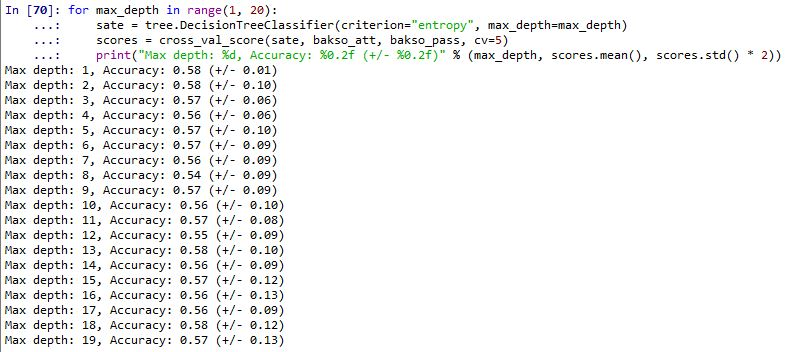
\includegraphics[scale=0.3]{figures/hasil10.jpg}
\caption{codingan ke-10}
\label{contoh}
\end{figure}

\end{itemize}
\par
\item Codingan Ke-11 :
\par Penjelasan : Codingan ini mendefinisikan bahwa variabel fadila akan mengeksekusi empty dari importan library numphy yang dinamakan np dengan 2 parameter yaitu 19,3 dan float. i didefinisikan dengan angka 0 kemudian untuk perhitungan jarak max depth diantara parameter 1 dan 20. Variabel sate mendefinisikan klasifikasi decision tree dengan 2 parameter. setelah itu, variabel score mendefinisikan variabel fadila dengan i dan 0, variabel kedua dari fadila dengan i dan 1 serta variabel ketiga dari fadila dengan i dan 2, maka pengeksekusian akhir bahwa variabel i akan ditambah dengan angka 1 untuk hasil akhirnya. Keluarannya akan berupa array dari perhitungan parameter dan variabel yang telah didefinisikan sebelumnya.
\par 
\begin{itemize}
\par
\item Hasil Codingan Ke-11 :

\begin{figure}[ht]
\centering
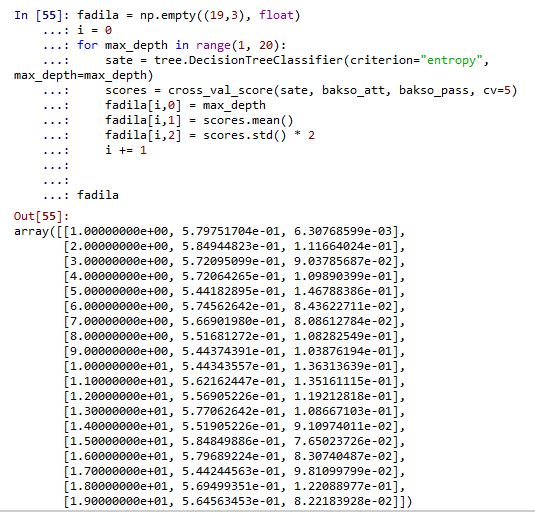
\includegraphics[scale=0.3]{figures/hasil11y.jpg}
\caption{codingan ke-11}
\label{contoh}
\end{figure}

\end{itemize}
\par
\item Codingan Ke-12 :
\par Penjelasan : Codingan ini mendefinisikan pemanggilan dari library matplotlib.pyplot sebagai fadila sehingga nanti hasilnya akan berbentuk gambar grafik/gelombang. Untuk variabel fig dan ax akan mendefinisikan subplots dari fadila. Setelah itu ketentuan dari parameter depth acc = 0, depth acc = 1 dan depth acc 2. Selanjutnya untuk menampilkan gelombang maka panggil variabel fadila dengan perintah show.
\par 
\begin{itemize}
\par
\item Hasil Codingan Ke-12 :

\begin{figure}[ht]
\centering
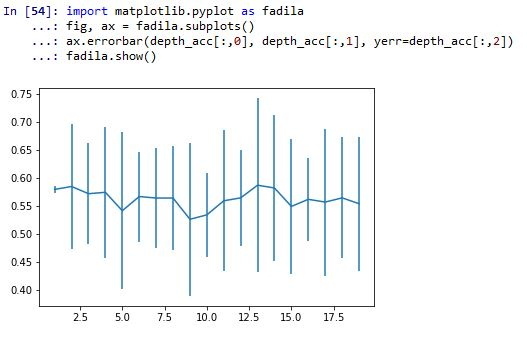
\includegraphics[scale=0.4]{figures/hasil12.jpg}
\caption{codingan ke-12}
\label{contoh}
\end{figure}

\end{itemize}
\end{enumerate}
\end{enumerate}

\subsection{Penanganan Error}
\par Pembahasan dan Penyelesaiian Error
\par
\begin{enumerate}
\item Error 1	: 
\par
\par

\begin{figure}[ht]
\centering
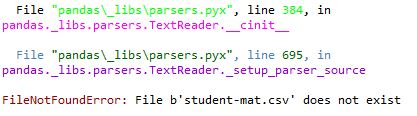
\includegraphics[scale=0.4]{figures/errorr.jpg}
\caption{error 1}
\label{contoh}
\end{figure}

\par
\begin{itemize}
\item Penjelasan	: 
\begin{itemize}
\item Pada error tersebut dikatakan bahwa untuk file -b"student-mat.csv" tidak ada. Mengapa? karena file codingan yang dieksekusi yaitu student-performance.py tidak berada pada folder yang sama jadi tidak dapat terpanggil dan tereksekusi.
\item Nah, untuk penyelesaiannya yaitu dengan menambahkan fungsi yang mendefinisikan folder tempat file "student-mat.csv berada. 
\item Silahkan tambahkan perintah " dataset/student-mat.csv " pada codingannya
\item Dengan penambahan perintah tersebut maka tidak akan terjadi error lagi.
\end{itemize}
\end{itemize}



\par
\item Error 2	:
\par

\begin{figure}[ht]
\centering
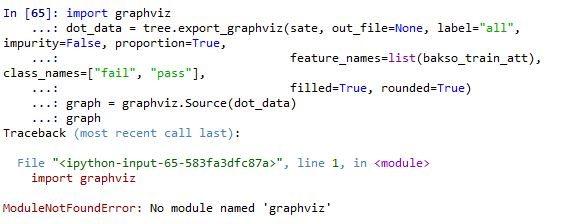
\includegraphics[scale=0.4]{figures/error6.jpg}
\caption{error 2}
\label{contoh}
\end{figure}


\par
\begin{itemize}
\item Penjelasan	: 
\begin{itemize}
\item Pada error tersebut dikatakan bahwa tidak terdapat module graphiz sehingga codingan tidak dapat dieksekusi.
\item Penanganannya yaitu dengan melakukan penginstalan module graphiz itu sendiri
\item Penginstalan bisa dilakukan pada Anaconda Prompt ataupun Command Prompt
\item Pada promt tersebut masukkan perintah " conda install graphviz "
\item Silahkan tunggu sampai instalasi berhasil
\item Setelah selesai, maka cobalah RUN kembali codingan terkait
\item Maka tidak akan terjadi error lagi.
\end{itemize}
\end{itemize}

\par
\item Error 3	:
\par

\begin{figure}[ht]
\centering
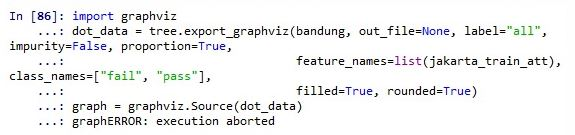
\includegraphics[scale=0.4]{figures/error62.jpg}
\caption{error 3}
\label{error 3}
\end{figure}

\par
\begin{itemize}
\item Penjelasan	: 
\begin{itemize}
\item Pada error tersebut dikatakan bahwa eksekusinya dilarang atau di aborted.
\item Penanganannya sebenarnya sederhana
\item Tidak terdapat kesalahan dalam pembuatan dan penyesuaian codingan 
\item Mungkin saja terjadi error tersebut karena pengeksekusian fungsi yang berulang-ulang pada codingan yang berbeda
\item Silahkan di Restart atau dijalankan kembali aplikasi spydernya
\item Run kembali maka errornya tidak akan muncul lagi dan hasilnya akan muncul seperti pada gambar pengujian no 6
\end{itemize}
\end{itemize}

\par
\item Error 4	:
\par

\begin{figure}[ht]
\centering
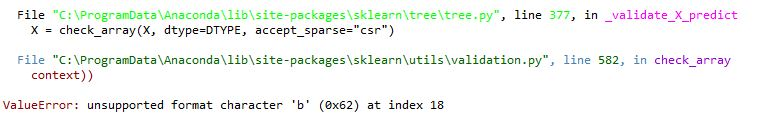
\includegraphics[scale=0.4]{figures/error8.jpg}
\caption{error 4}
\label{contoh}
\end{figure}

\par

\par
\begin{itemize}
\item Penjelasan	: 
\begin{itemize}
\item Pada error tersebut dikatakan terdapat error karakter b nya gak kebaca
\item Penanganannya sebenarnya sederhana, dari codingan tidak ada yang salah
\item Disarankan agar mengulang kembali penamaan untuk variabel terkait dari awal codingan hingga akhir sehingga lebih teratur
\item Silahkan dicoba run codingan tersebut kembali
\item Maka codingannya akan berhasil dan muncul seperti pada contoh codingan no 8 diatas
\end{itemize}
\end{itemize}

\end{enumerate}
\end{enumerate}

\section{Lusia Violita Aprilian}
\subsection{binary classification dilengkapi ilustrasi gambar}

\par Binary classification yaitu berupa kelas positif dan kelas negatif. Klasifikasi biner adalah dikotomisasi yang diterapkan untuk tujuan praktis, dan dalam banyak masalah klasifikasi biner praktis, kedua kelompok tidak simetris - daripada akurasi keseluruhan, proporsi relatif dari berbagai jenis kesalahan yang menarik. Misalnya, dalam pengujian medis, false positive (mendeteksi penyakit ketika tidak ada) dianggap berbeda dari false negative (tidak mendeteksi penyakit ketika hadir).

\begin{figure}[ht]
\centering
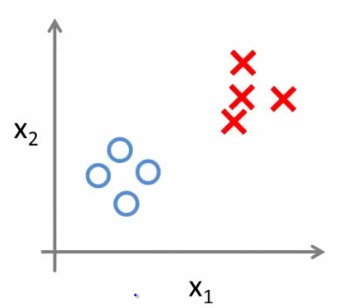
\includegraphics[scale=0.5]{figures/f1.jpg}
\caption{Binary Classification}
\label{contoh}
\end{figure}

\subsection{supervised learning dan unsupervised learning dan clustering\\ dengan ilustrasi gambar}

\begin{enumerate}

\item Supervised learning adalah tugas pembelajaran mesin untuk mempelajari suatu fungsi yang memetakan input ke output berdasarkan contoh pasangan input-output. Ini menyimpulkan fungsi dari data pelatihan berlabel yang terdiri dari serangkaian contoh pelatihan. Dalam pembelajaran yang diawasi, setiap contoh adalah pasangan yang terdiri dari objek input (biasanya vektor) dan nilai output yang diinginkan (juga disebut sinyal pengawas). Algoritma pembelajaran yang diawasi menganalisis data pelatihan dan menghasilkan fungsi yang disimpulkan, yang dapat digunakan untuk memetakan contoh-contoh baru. Skenario optimal akan memungkinkan algoritma menentukan label kelas dengan benar untuk instance yang tidak terlihat. Ini membutuhkan algoritma pembelajaran untuk menggeneralisasi dari data pelatihan untuk situasi yang tidak terlihat dengan cara yang "masuk akal" (lihat bias induktif). Tugas paralel dalam psikologi manusia dan hewan sering disebut sebagai pembelajaran konsep.

\begin{figure}[ht]
\centering
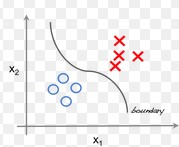
\includegraphics[scale=0.5]{figures/f2.jpg}
\caption{Supervised Learning}
\label{contoh}
\end{figure}

\item Unsupervised learning adalah istilah yang digunakan untuk pembelajaran bahasa Ibrani, yang terkait dengan pembelajaran tanpa guru, juga dikenal sebagai organisasi mandiri dan metode pemodelan kepadatan probabilitas input. Analisis cluster sebagai cabang pembelajaran mesin yang mengelompokkan data yang belum diberi label, diklasifikasikan atau dikategorikan. Alih-alih menanggapi umpan balik, analisis klaster mengidentifikasi kesamaan dalam data dan bereaksi berdasarkan ada tidaknya kesamaan di setiap potongan data baru.

\begin{figure}[ht]
\centering
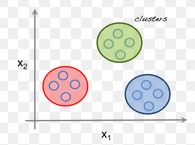
\includegraphics[scale=0.5]{figures/f3.jpg}
\caption{Unsupervised Learning}
\label{contoh}
\end{figure}

\item Cluster analysis or clustering adalah tugas pengelompokan sekumpulan objek sedemikian rupa sehingga objek dalam kelompok yang sama (disebut klaster) lebih mirip (dalam beberapa hal) satu sama lain daripada pada kelompok lain (kluster). Ini adalah tugas utama penambangan data eksplorasi, dan teknik umum untuk analisis data statistik, yang digunakan di banyak bidang, termasuk pembelajaran mesin, pengenalan pola, analisis gambar, pengambilan informasi, bioinformatika, kompresi data, dan grafik komputer. Analisis Cluster sendiri bukan merupakan salah satu algoritma spesifik, tetapi tugas umum yang harus dipecahkan. Ini dapat dicapai dengan berbagai algoritma yang berbeda secara signifikan dalam pemahaman mereka tentang apa yang merupakan sebuah cluster dan bagaimana cara menemukannya secara efisien. Gagasan populer mengenai cluster termasuk kelompok dengan jarak kecil antara anggota cluster, area padat ruang data, interval atau distribusi statistik tertentu. Clustering karena itu dapat dirumuskan sebagai masalah optimasi multi-objektif. Algoritma pengelompokan dan pengaturan parameter yang sesuai (termasuk parameter seperti fungsi jarak yang akan digunakan, ambang kepadatan atau jumlah cluster yang diharapkan) tergantung pada set data individual dan penggunaan hasil yang dimaksudkan. Analisis kluster bukan merupakan tugas otomatis, tetapi proses berulang penemuan pengetahuan atau optimasi multi-objektif interaktif yang melibatkan percobaan dan kegagalan. Seringkali diperlukan untuk memodifikasi praproses data dan parameter model hingga hasilnya mencapai properti yang diinginkan.

\begin{figure}[ht]
\centering
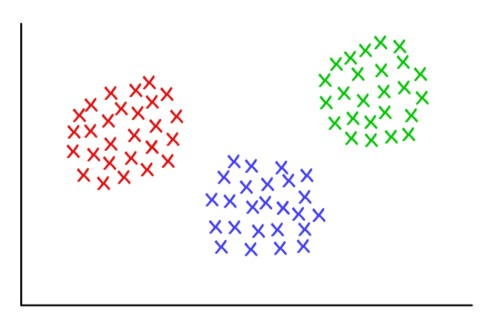
\includegraphics[scale=0.5]{figures/f4.jpg}
\caption{Cluster}
\label{contoh}
\end{figure}

\end{enumerate}

\subsection{evaluasi dan akurasi dari buku dan disertai ilustrasi contoh
dengan gambar}

\par Evaluasi adalah tentang bagaimana kita dapat mengevaluasi seberapa baik model bekerja dengan mengukur akurasinya. Dan akurasi akan didefinisikan sebagai persentase kasus yang diklasifikasikan dengan benar. Kita dapat menganalisis kesalahan yang dibuat oleh model, atau tingkat kebingungannya, menggunakan matriks kebingungan. Matriks kebingungan mengacu pada kebingungan dalam model, tetapi matriks kebingungan ini bisa menjadi sedikit sulit untuk dipahami ketika mereka menjadi sangat besar.

\begin{figure}[ht]
\centering
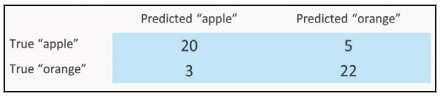
\includegraphics[scale=0.5]{figures/f9.jpg}
\caption{ Evaluasi dan Akurasi}
\label{contoh}
\end{figure}

\subsection{ bagaimana cara membuat dan membaca confusion matrix, buat confusion matrix }
\begin{enumerate}
\item Cara membuat dan membaca confusion matrix :
\begin{enumerate}
\item Tentukan pokok permasalahan dan atributanya, misal gaji dan listik.
\item Buat pohon keputusan
\item Lalu data testingnya
\item Lalu mencari nilai a, b, c, dan d. Semisal a = 5, b = 1, c = 1, dan d = 3.
\item Selanjutnya mencari nilai recall, precision, accuracy, serta dan error rate.
\end{enumerate}

\item Berikut adalah contoh dari confusion matrix :
\begin{itemize}
\item Recall =3/(1+3) = 0,75
\item Precision = 3/(1+3) = 0,75
\item Accuracy =(5+3)/(5+1+1+3) = 0,8
\item Error Rate =(1+1)/(5+1+1+3) = 0,2
\end{itemize}
\end{enumerate}


\subsection{bagaimana K-fold cross validation bekerja dengan gambar ilustrasi}

\par Cara kerja K-fold cross validation :
\begin{enumerate}
\item Total instance dibagi menjadi N bagian.
\item Fold yang pertama adalah bagian pertama menjadi data uji (testing data) dan sisanya menjadi training data.
\item Lalu hitung akurasi berdasarkan porsi data tersebut dengan menggunakan persamaan.
\item Fold yang ke dua adalah bagian ke dua menjadi data uji (testing data) dan sisanya training data. 
\item Kemudian hitung akurasi berdasarkan porsi data tersebut.
\item Dan seterusnya hingga habis mencapai fold ke-K.
\item Terakhir hitung rata-rata akurasi K buah.
\end{enumerate}



\begin{figure}[ht]
\centering
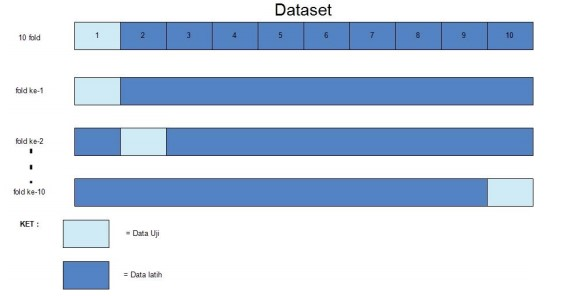
\includegraphics[scale=0.5]{figures/f5.jpg}
\caption{K-fold cross validation }
\label{contoh}
\end{figure}

\subsection{decision tree dengan gambar ilustrasi}

\par Decision tree adalah model visual yang terdiri dari node dan cabang, seperti Gambar dijelaskan secara rinci nanti dalam artikel ini. Untuk saat ini, amati bahwa ia tumbuh dari kiri ke kanan, dimulai dengan simpul keputusan root (kuadrat, juga disebut simpul pilihan) yang cabang-cabangnya mewakili dua atau lebih opsi bersaing yang tersedia bagi para pembuat keputusan. Pada akhir cabang awal ini, ada simpul akhir (segitiga, juga disebut simpul nilai) atau simpul ketidakpastian (lingkaran, juga disebut simpul peluang). Node akhir mewakili nilai tetap. Cabang lingkaran mewakili hasil yang mungkin bersama dengan probabilitasnya masing-masing (yang berjumlah 1,0). Di luar cabang-cabang node ketidakpastian awal ini, mungkin ada lebih banyak bujur sangkar dan lebih banyak lingkaran, yang umumnya bergantian sampai setiap jalur berakhir di simpul akhir.

\begin{figure}[ht]
\centering
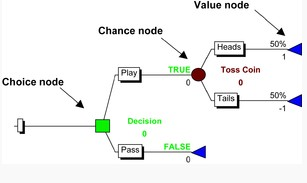
\includegraphics[scale=0.5]{figures/f6.jpg}
\caption{Decision Tree}
\label{contoh}
\end{figure}

\subsection{Information gain dan entropi dengan gambar ilustrasi}

\begin{enumerate}
\item Information gain (IG) mengukur seberapa banyak informasi fitur memberi kita tentang kelas. - Fitur yang sempurna mempartisi harus memberikan informasi maksimal. - Fitur yang tidak terkait seharusnya tidak memberikan informasi.

\begin{figure}[ht]
\centering
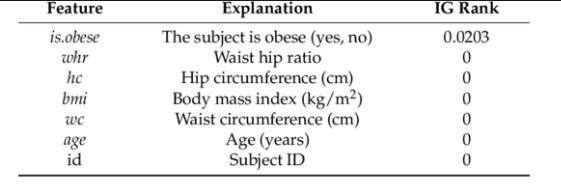
\includegraphics[scale=0.5]{figures/f7.jpg}
\caption{Information gain}
\label{contoh}
\end{figure}

\item Entropi merupakan kemurnian dalam koleksi contoh yang sewenang-wenang.

\begin{figure}[ht]
\centering
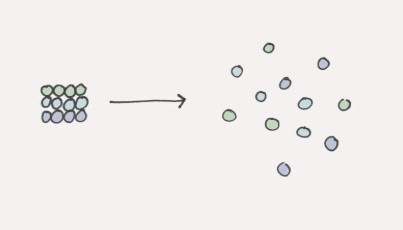
\includegraphics[scale=0.5]{figures/f8.jpg}
\caption{Entropi}
\label{contoh}
\end{figure}
\end{enumerate}

\subsection{binary classification dilengkapi ilustrasi gambar}

\par Binary classification yaitu berupa kelas positif dan kelas negatif. Klasifikasi biner adalah dikotomisasi yang diterapkan untuk tujuan praktis, dan dalam banyak masalah klasifikasi biner praktis, kedua kelompok tidak simetris - daripada akurasi keseluruhan, proporsi relatif dari berbagai jenis kesalahan yang menarik. Misalnya, dalam pengujian medis, false positive (mendeteksi penyakit ketika tidak ada) dianggap berbeda dari false negative (tidak mendeteksi penyakit ketika hadir).

\begin{figure}[ht]
\centering
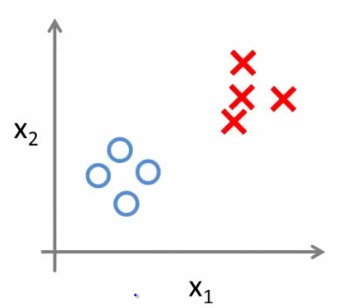
\includegraphics[scale=0.5]{figures/f1.jpg}
\caption{Binary Classification}
\label{contoh}
\end{figure}

\subsection{supervised learning dan unsupervised learning dan clustering\\ dengan ilustrasi gambar}

\begin{enumerate}
\item Supervised learning adalah tugas pembelajaran mesin untuk mempelajari suatu fungsi yang memetakan input ke output berdasarkan contoh pasangan input-output. Ini menyimpulkan fungsi dari data pelatihan berlabel yang terdiri dari serangkaian contoh pelatihan. Dalam pembelajaran yang diawasi, setiap contoh adalah pasangan yang terdiri dari objek input (biasanya vektor) dan nilai output yang diinginkan (juga disebut sinyal pengawas). Algoritma pembelajaran yang diawasi menganalisis data pelatihan dan menghasilkan fungsi yang disimpulkan, yang dapat digunakan untuk memetakan contoh-contoh baru. Skenario optimal akan memungkinkan algoritma menentukan label kelas dengan benar untuk instance yang tidak terlihat. Ini membutuhkan algoritma pembelajaran untuk menggeneralisasi dari data pelatihan untuk situasi yang tidak terlihat dengan cara yang "masuk akal" (lihat bias induktif). Tugas paralel dalam psikologi manusia dan hewan sering disebut sebagai pembelajaran konsep.

\begin{figure}[ht]
\centering
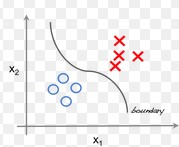
\includegraphics[scale=0.5]{figures/f2.jpg}
\caption{Supervised Learning}
\label{contoh}
\end{figure}

\item Unsupervised learning adalah istilah yang digunakan untuk pembelajaran bahasa Ibrani, yang terkait dengan pembelajaran tanpa guru, juga dikenal sebagai organisasi mandiri dan metode pemodelan kepadatan probabilitas input. Analisis cluster sebagai cabang pembelajaran mesin yang mengelompokkan data yang belum diberi label, diklasifikasikan atau dikategorikan. Alih-alih menanggapi umpan balik, analisis klaster mengidentifikasi kesamaan dalam data dan bereaksi berdasarkan ada tidaknya kesamaan di setiap potongan data baru.

\begin{figure}[ht]
\centering
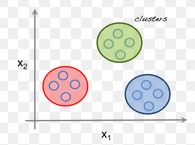
\includegraphics[scale=0.5]{figures/f3.jpg}
\caption{Unsupervised Learning}
\label{contoh}
\end{figure}

\item Cluster analysis or clustering adalah tugas pengelompokan sekumpulan objek sedemikian rupa sehingga objek dalam kelompok yang sama (disebut klaster) lebih mirip (dalam beberapa hal) satu sama lain daripada pada kelompok lain (kluster). Ini adalah tugas utama penambangan data eksplorasi, dan teknik umum untuk analisis data statistik, yang digunakan di banyak bidang, termasuk pembelajaran mesin, pengenalan pola, analisis gambar, pengambilan informasi, bioinformatika, kompresi data, dan grafik komputer. Analisis Cluster sendiri bukan merupakan salah satu algoritma spesifik, tetapi tugas umum yang harus dipecahkan. Ini dapat dicapai dengan berbagai algoritma yang berbeda secara signifikan dalam pemahaman mereka tentang apa yang merupakan sebuah cluster dan bagaimana cara menemukannya secara efisien. Gagasan populer mengenai cluster termasuk kelompok dengan jarak kecil antara anggota cluster, area padat ruang data, interval atau distribusi statistik tertentu. Clustering karena itu dapat dirumuskan sebagai masalah optimasi multi-objektif. Algoritma pengelompokan dan pengaturan parameter yang sesuai (termasuk parameter seperti fungsi jarak yang akan digunakan, ambang kepadatan atau jumlah cluster yang diharapkan) tergantung pada set data individual dan penggunaan hasil yang dimaksudkan. Analisis kluster bukan merupakan tugas otomatis, tetapi proses berulang penemuan pengetahuan atau optimasi multi-objektif interaktif yang melibatkan percobaan dan kegagalan. Seringkali diperlukan untuk memodifikasi praproses data dan parameter model hingga hasilnya mencapai properti yang diinginkan.

\begin{figure}[ht]
\centering
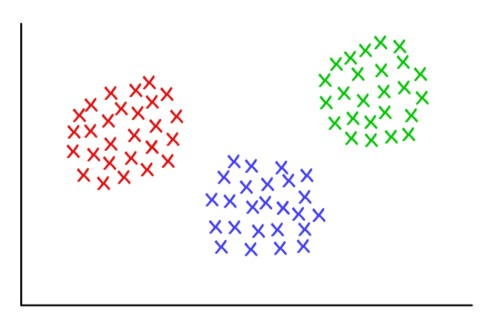
\includegraphics[scale=0.5]{figures/f4.jpg}
\caption{Cluster}
\label{contoh}
\end{figure}

\end{enumerate}

\subsection{evaluasi dan akurasi dari buku dan disertai ilustrasi contoh\\ dengan gambar}

\par Evaluasi adalah tentang bagaimana kita dapat mengevaluasi seberapa baik model bekerja dengan mengukur akurasinya. Dan akurasi akan didefinisikan sebagai persentase kasus yang diklasifikasikan dengan benar. Kita dapat menganalisis kesalahan yang dibuat oleh model, atau tingkat kebingungannya, menggunakan matriks kebingungan. Matriks kebingungan mengacu pada kebingungan dalam model, tetapi matriks kebingungan ini bisa menjadi sedikit sulit untuk dipahami ketika mereka menjadi sangat besar.

\begin{figure}[ht]
\centering
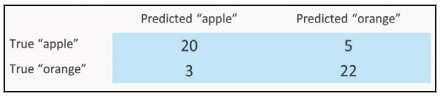
\includegraphics[scale=0.5]{figures/f9.jpg}
\caption{ Evaluasi dan Akurasi}
\label{contoh}
\end{figure}

\subsection{ bagaimana cara membuat dan membaca confusion matrix, buat confusion matrix }
\begin{enumerate}
\item Cara membuat dan membaca confusion matrix :
\begin{enumerate}
\item 1) Tentukan pokok permasalahan dan atributanya, misal gaji dan listik.
\item 2) Buat pohon keputusan
\item 3) Lalu data testingnya
\item 4) Lalu mencari nilai a, b, c, dan d. Semisal a = 5, b = 1, c = 1, dan d = 3.
\item 5) Selanjutnya mencari nilai recall, precision, accuracy, serta dan error rate.
\end{enumerate}

\item Berikut adalah contoh dari confusion matrix :
\begin{itemize}
\item Recall =3/(1+3) = 0,75
\item Precision = 3/(1+3) = 0,75
\item Accuracy =(5+3)/(5+1+1+3) = 0,8
\item Error Rate =(1+1)/(5+1+1+3) = 0,2
\end{itemize}
\end{enumerate}


\subsection{bagaimana K-fold cross validation bekerja dengan gambar ilustrasi}

\par Cara kerja K-fold cross validation :
\begin{enumerate}
\item Total instance dibagi menjadi N bagian.
\item Fold yang pertama adalah bagian pertama menjadi data uji (testing data) dan sisanya menjadi training data.
\item Lalu hitung akurasi berdasarkan porsi data tersebut dengan menggunakan persamaan.
\item Fold yang ke dua adalah bagian ke dua menjadi data uji (testing data) dan sisanya training data. 
\item Kemudian hitung akurasi berdasarkan porsi data tersebut.
\item Dan seterusnya hingga habis mencapai fold ke-K.
\item Terakhir hitung rata-rata akurasi K buah.
\end{enumerate}

\begin{figure}[ht]
\centering
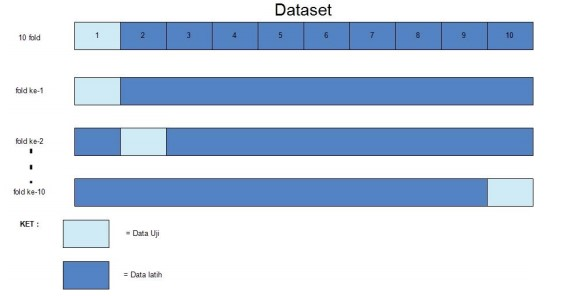
\includegraphics[scale=0.5]{figures/f5.jpg}
\caption{K-fold cross validation }
\label{contoh}
\end{figure}

\subsection{decision tree dengan gambar ilustrasi}

\par Decision tree adalah model visual yang terdiri dari node dan cabang, seperti Gambar dijelaskan secara rinci nanti dalam artikel ini. Untuk saat ini, amati bahwa ia tumbuh dari kiri ke kanan, dimulai dengan simpul keputusan root (kuadrat, juga disebut simpul pilihan) yang cabang-cabangnya mewakili dua atau lebih opsi bersaing yang tersedia bagi para pembuat keputusan. Pada akhir cabang awal ini, ada simpul akhir (segitiga, juga disebut simpul nilai) atau simpul ketidakpastian (lingkaran, juga disebut simpul peluang). Node akhir mewakili nilai tetap. Cabang lingkaran mewakili hasil yang mungkin bersama dengan probabilitasnya masing-masing (yang berjumlah 1,0). Di luar cabang-cabang node ketidakpastian awal ini, mungkin ada lebih banyak bujur sangkar dan lebih banyak lingkaran, yang umumnya bergantian sampai setiap jalur berakhir di simpul akhir.
\begin{figure}[ht]
\centering
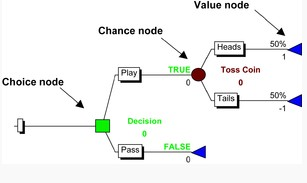
\includegraphics[scale=0.5]{figures/f6.jpg}
\caption{Decision Tree}
\label{contoh}
\end{figure}

\subsection{Information gain dan entropi dengan gambar ilustrasi}
\begin{enumerate}
\item Information gain (IG) mengukur seberapa banyak "informasi" fitur memberi kita tentang kelas. - Fitur yang sempurna mempartisi harus memberikan informasi maksimal. - Fitur yang tidak terkait seharusnya tidak memberikan informasi.
\begin{figure}[ht]
\centering
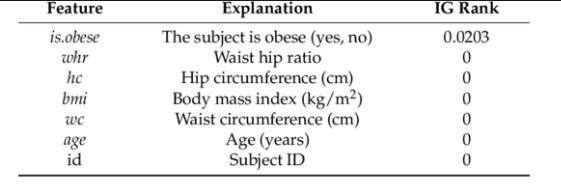
\includegraphics[scale=0.5]{figures/f7.jpg}
\caption{Information gain}
\label{contoh}
\end{figure}

\item Entropi merupakan kemurnian dalam koleksi contoh yang sewenang-wenang.
\begin{figure}[ht]
\centering
\includegraphics[scale=0.7]{figures/f8.jpg}
\caption{Entropi}
\label{contoh}
\end{figure}

\end{enumerate}

\subsection{scikit-learn}
\begin{enumerate}

\item load dataset 
\begin{figure}
\centering
\includegraphics[scale=0.9]{figures/g1.jpg}
\caption{load dataset}
\label{contoh}
\end{figure}
\par Pada gambar tersebut dijelaskan bahwa in dengan mengimport pandas dengan diperumpamakan sebagai pd. Pada baris ke dua, dibuat variable nanas untuk memanggil pd sehingga dapat membaca file csv. Dan pada baris ke 3 variable dipanggil. Sehingga menghasilkan output 395. 

\item generate binary label (pass/fail) based on G1+G2+G3 
\begin{figure}
\centering
\includegraphics[scale=0.5]{figures/g2.jpg}
\caption{generate binary label}
\label{contoh}
\end{figure}
\par Pada gambar tersebut dijelaskan bahwa in pada baris pertama, dibuat variable nanas untuk memanggil nanas dengan apply lamda sehingga baris selanjutnya nanas meng-drop G1, G2, dan G3. Dan pada baris ke 3 variable dipanggil. Sehingga menghasilkan output sebuah data 5 rows x 31 columns.

\item  use one-hot encoding on categorical columns 
\begin{figure}
\centering
\includegraphics[scale=0.5]{figures/g3.jpg}
\caption{use one-hot encoding on categorical columns}
\label{contoh}
\end{figure}
\par Pada gambar tersebut dijelaskan bahwa in pada baris pertama, dibuat variable nanas untuk memanggil pd dengan get dummies nanas columns. Dan pada baris selanjutnya variable dipanggil. Sehingga menghasilkan output sebuah data 5 rows x 57 columns.

\item shuffle rows,  split training dan testing data 
\begin{figure}
\centering
\includegraphics[scale=0.5]{figures/g4.jpg}
\caption{shuffle rows, split training dan testing data}
\label{contoh}
\end{figure}
\par Pada gambar tersebut dijelaskan bahwa in pada baris pertama, dibuat variable nanas untuk memanggil nanas sebagai sample. Lalu pada baris selanjutnya dilakukan split training dan testing data. Setelah data dilakukan split training da testing, import file numpy sebagai np dan kemudian melakukan prerintah print. Sehingga menghasilkan passing: 116 out of 395.

\item fit a decision tree
\begin{figure}
\centering
\includegraphics[scale=0.5]{figures/g5.jpg}
\caption{fit a decision tree}
\label{contoh}
\end{figure}
\par Pada gambar tersebut dijelaskan bahwa in pada baris pertama, import tree dari sklearn. Pada baris selanjutnya variable duku memanggil tree dengan decision tree clasisifier dengan criteria entropy dan max dept = 5. Dan pada baris terakhir, variable duku memanggil duku dengan fit nanas train att dan nanas train pass.

\item visualize tree 
\begin{figure}
\centering
\includegraphics[scale=0.5]{figures/g6a.jpg}
\caption{visualize tree}
\label{contoh}
\end{figure}
\par Pada gambar tesebut menjelaskan import graphviz dengan variabelm dot data, class name, class name, dan graph. Sehingga menampilkan gambar sebagai berikut :
\begin{figure}
\centering
\includegraphics[scale=0.5]{figures/g6b.jpeg}
\caption{visualize tree}
\label{contoh}
\end{figure}


\item save tree
\begin{figure}
\centering
\includegraphics[scale=0.5]{figures/g7.jpg}
\caption{save tree}
\label{contoh}
\end{figure}
\par Pada gambar tersebut dijelaskan bahwa in pada baris pertama, Tree export graphviz duku dengan out file student-performance.dot dan label all. pada baris selanjutnya dijelaskan featura names = list dan class name fail atau pas. Apabila bernilai true akan filled dan rounded.
 
\item t.score
\begin{figure}
\centering
\includegraphics[scale=0.5]{figures/g8.jpg}
\caption{t.score}
\label{contoh}
\end{figure}
\par Pada gambar tersebut dijelaskan bahwa in pada baris pertama, parameter dengan hasilnya adalah duku.score yang dimana terdapat perhitungan nanas test at dan nana test pass.


\item show average score and +/- two standard deviations away 
\begin{figure}
\centering
\includegraphics[scale=0.5]{figures/g9.jpg}
\caption{show average score}
\label{contoh}
\end{figure}
\par Pada gambar tersebut dijelaskan bahwa in pada baris pertama memanggil cross vla score dari sklearn.model selection. Pada baris selanjutnya membuat variabel scores. Dan pada baris terakhir score akan ditampilkan.

\item for max depth in range 
\begin{figure}
\centering
\includegraphics[scale=0.5]{figures/g10.jpg}
\caption{for max depth in range}
\label{contoh}
\end{figure}
\par Pada gambar tersebut dijelaskan bahwa in pada baris pertama mendefinisikan range dari 1 hinga 20. Lalu, variabel duku memdefinisikan tree dengan decision tree clasification kriteria entropy. Dan variable scores mendefinisikan duku, nanas att, nanas pass dan cv = 5. Baris terakhir adalah menampilkan hasil.

\item depth acc
\begin{figure}
\centering
\includegraphics[scale=0.5]{figures/g11.jpg}
\caption{depth acc}
\label{contoh}
\end{figure}
\par Pada gambar tersebut dijelaskan bahwa variabel depth acc mendefinisikan np empty dengan i = 0 dari range 1-20. Dimana pada range tersebut terdapat variabel duku dan score. Variabel duku memdefinisikan tree dengan decision tree clasification kriteria entropy. Dan variable scores mendefinisikan duku, nanas att, nanas pass dan cv = 5. Dan pada baris selanjutnya adalah pendefinisian depth acc. Sehingga didapatlah hasil berupa array.

\item matplotlib
\begin{figure}
\centering
\includegraphics[scale=0.5]{figures/g12.jpg}
\caption{matplotlib}
\label{contoh}
\end{figure}
\par Pada gambar tersebut dijelaskan bahwa in pada baris pertama mendefinisikan pemanggilan  matplotlib.pyplot sebagai plt. Lalu pendefinisian figure dari plt serta error bar. Dan pada baris terakhir menampilkan plt. Maka akan muncul sebuah gambar berupa giagram.

\end{enumerate}

\subsection{Penanganan Error}
\begin{enumerate}
\item Skrinsut error
\begin{figure}
\centering
\includegraphics[scale=0.5]{figures/h1.jpg}
\caption{error}
\label{contoh}
\end{figure}

\item Tuliskan kode eror dan jenis errornya
\par Kode dan jenis error yang didapatkan adalah :
\begin{itemize}
\item Kode error = FileNotFoundError: File b'student-por.csv' does not exist
\item Jenis error = FileNotFoundError
\end{itemize}

\item Solusi pemecahan masalah error tersebut
\par Berikut adalah solusi dari permasalahan pada no. 1
\begin{figure}
\centering
\includegraphics[scale=0.5]{figures/g1.jpg}
\caption{penyelesaian}
\label{contoh}
\end{figure}

\end{enumerate}



\section{Rahmi Roza/1164085}
\subsection{Teori}
Penyelesaian Tugas Harian 3 ( No. 1-7 )
\begin{enumerate}
\item Binary Classification Dan Ilustrasi Gambarnya
\begin{itemize}
\item Pengertian Binary Classification / Klasifikasi Biner:
\par Klasifikasi biner atau binomial adalah tugas mengklasifikasikan elemen-elemen dari himpunan yang diberikan ke dalam dua kelompok (memprediksi kelompok mana yang masing-masing dimiliki) berdasarkan aturan klasifikasi.
\item Ilustrasi Gambar Binary Classification :
\par

\begin{figure}[ht]
\centering
\includegraphics[scale=0.7]{figures/gambar1.PNG}
\caption{binary classification}
\label{gambar1}
\end{figure}

\par
\item Supervised Learning, Unsupervised Learning, Clustering Dan Ilustrasi Gambar
\begin{itemize}
\item Pengertian Supervised Learning :
\par Supervised learning adalah sebuah pendekatan dimana sudah terdapat data yang dilatih, dan terdapat variable yang ditargetkan sehingga tujuan dari pendekatan ini adalah mengkelompokan suatu data ke data yang sudah ada.
\end{itemize}
\par
\item Ilustrasi Gambar Supervised Learning :

\begin{figure}[ht]
\centering
\includegraphics[scale=0.7]{figures/gambar2.JPG}
\caption{supervised}
\label{gambar2}
\end{figure}

\item Pengertian Unsupervised Learning :
\par unsupervised learning tidak memiliki data latih, sehingga dari data yang ada, kita mengelompokan data tersebut menjadi 2 bagian atau 3 bagian dan seterusnya.
\par
\par
\begin{itemize}
\item Ilustrasi Gambar Unsupervised Learning :

\begin{figure}[ht]
\centering
\includegraphics[scale=0.7]{figures/gambar3.JPG}
\caption{unsupervised}
\label{gambar3}
\end{figure}
\end{itemize}

\item Pengertian Clustering :
\par Metode pengelompokan data. Clustering juga merupakan proses partisi satu set objek data ke dalam himpunan bagian yang disebut dengan cluster. Objek dalam cluster tersebut memiliki kemiripan karakteristik antar satu sama lain.
\par

\begin{figure}[ht]
\centering
\includegraphics[scale=0.5]{figures/gambar4.JPG}
\caption{clustering}
\label{gambar4}
\end{figure}

\par
\end{itemize}
\item Evaluasi, Akurasi Dan Ilustrasi Gambar
\begin{itemize}
\item Pengertian Evaluasi
\par Evaluasi digunakan untuk memeriksa/memastikan dan mengevaluasi model dalam bekerja ( seberapa baik ) dengan mengukur keakuratannya. Kita juga dapat menanalisis kesalahan yang dibuat pada model yang dijalankan, tingkat kebingungan dan menggunakan matriks kebingunan.
\par

\begin{figure}[ht]
\centering
\includegraphics[scale=0.7]{figures/gambar5.JPG}
\caption{Evaluasi}
\label{gambar5}
\end{figure}


\par
\item Pengertian Akurasi
\par Accuracy akan didefinisikan sebagai presentasi kasus yang diklasifikasikan dengan benar. Accuracy lebih jelasnya adalah perbandingan kasus yang diidentifikasi benar dengan jumlah semua kasus
\par Rumus dari accuracy= (a+c)/(a+b+c+d)
\par

\begin{figure}[ht]
\centering
\includegraphics[scale=0.8]{figures/acuracy.jpg}
\caption{Akurasi}
\label{contoh}
\end{figure}

\par Dilakukan perhitungan dengan rumus akurasi terhadap data yang telah diolah pada " Evaluasi ". Kemudian di dapatkan hasil dari pengolahan data tersebut.
\par Contoh penggabungan Akurasi Dan Evaluasi
\par

\begin{figure}[ht]
\centering
\includegraphics[scale=0.5]{figures/evacuray.jpg}
\caption{Contoh Evaluasi Dan Akurasi Secara Bersamaan }
\label{contoh}
\end{figure}

\end{itemize}

\par
\item Membuat Dan Membaca Confusion Matrix Beserta Contoh
\begin{itemize}
\item Pengertian Confusion Matrix
\par Confusion matrix adalah suatu metode yang biasanya digunakan untuk melakukan perhitungan akurasi pada konsep data mining. Rumus ini melakukan perhitungan dengan 4 keluaran, yaitu: recall, precision, acuraccy dan error rate.
\par
\item Pembacaan Confusion Matrix
\begin{enumerate}
\item Apabila hasil prediksi negatif dan data sebenarnya merupakan negatif.
\item Apabila hasil prediksi positif sedangkan nilai sebenarnya merupakan negatif.
\item Apabila hasil prediksi negatif sedangkan nilai sebenarnya merupakan positif.
\item Apabila hasil prediksi positif dan nilai sebenarnya merupakan positif.
\end{enumerate}
\par
\par
\item Pembuatan Confusion Matrix
\begin{enumerate}
\item Menentukan 4 proses klasifikasi yang akan digunakan dalam confusion matrix.
\item 4 Istilah tersebut ada True Positive ( TP ), True Negative ( TN ), False Positive ( FP ) dan False Negative ( FN ).
\item Kelompokkan klasifikasi tersebut bisa menggunakan klasifikasi biner
\item Akan menghasilkan keluaran berupa 2 Kelas ( Positif dan Negatif ) dan penentuan TP, FP ( 1 klasifikasi positif ) , FN dan TN ( 1 klasifikasi negatif ).
\item Contoh dasarnya nampak seperti langkah diatas
\item Istilahnya daat didefinisikan dengan objek lain namu dengan alur yang sama ( sesuai rumus baik klasifikasi dll ).
\end{enumerate}
\par

\item Ilustrasi Gambar
\par

\begin{figure}[ht]
\centering
\includegraphics[scale=0.6]{figures/gambar6.PNG}
\caption{confusion matrix}
\label{gambar6}
\end{figure}
\end{itemize}

\par
\item Cara Kerja K-Fold Classification Dan Ilustrasi Gambar
\begin{enumerate}
\item Pertama-tama untuk total instance dibagi menjadi N bagian.
\item Fold ke-1 ( atau pertama ) adalah ketika bagian ke-1 menjadi data uji (testing data) dan sisanya menjadi data latih (training data).
\item Hitung akurasi ( berdasarkan porsi data tersebut. Persamaanya sebagai berikut :
\par (sigma) data klasifikasi
\par (sigma) total data uji
\par x 100 persen 
\item Fold ke-2 ( kedua ) adalah ketika bagian ke-2 menjadi data uji (testing data) dan sisanya menjadi data latih (training data). 
\item Kemudian dihitunglah akurasi berdasarkan porsi data yang telah ditentukan
\item Demikian seterusnya hingga mencapai fold ke-K. Hitung rata-rata akurasi dari K buah akurasi di atas. Rata-rata akurasi ini menjadi akurasi final atau akhir.
\end{enumerate}
\par
\begin{itemize}
\item Ilustrasi Gambar
\par

\begin{figure}[ht]
\centering
\includegraphics[scale=0.7]{figures/gambar7.PNG}
\caption{k-fold classification 1}
\label{gambar7}
\end{figure}

\par
\item Decision Tree Dan Ilustrasi Gambar
\begin{itemize}
\item Pengertian Decision Tree
\par Decision Tree (Pohon Keputusan) adalah pohon dimana setiap cabangnyamenunjukkan pilihan diantara sejumlah alternatif pilihan yang ada, dan setiapdaunnya menunjukkan keputusan yang dipilih.Decision tree biasa digunakan untuk mendapatkan informasi untuk tujuanpengambilan sebuah keputusan. Decision tree dimulai dengan sebuah root node(titik awal) yang dipakai oleh user untuk mengambil tindakan. Dari node root ini,user memecahnya sesuai dengan algoritma decision tree. Hasil akhirnya adalahsebuah decision tree dengan setiap cabangnya menunjukkan kemungkinansekenario dari keputusan yang diambil serta hasilnya.
\par

\end{itemize}
\par

\par
\begin{itemize}
\item Ilustrasi Gambar
\par


\begin{figure}[ht]
\centering
\includegraphics[scale=0.5]{figures/gambar8.JPG}
\caption{decision tree}
\label{gambar8}
\end{figure}

\par
\end{itemize}
\item Information Gain Dan Entropi
\begin{itemize}
\item Pengertian Information Gain
\par Information gain adalah salah satu atribute selection measure yang digunakan untuk memilih test atribute tiap node pada tree. Atribut dengan information gain tertinggi dipilih sebagai test atribut dari suatu node. Ada 2 kasus berbeda pada saat penghitungan Information Gain, pertama untuk kasus penghitungan atribut tanpa missing value dan kedua, penghitungan atribut dengan missing value.
\par

\end{itemize}
\item Ilustrasi Gambar
\par


\begin{figure}[ht]
\centering
\includegraphics[scale=0.3]{figures/gambar9.PNG}
\caption{informaion gain 1}
\label{gambar9}
\end{figure}


\par
\item Pengertian Entropi
\par Adalah suatu parameter untuk mengukur tingkat keberagaman (heterogenitas) dari kumpulan data. Semakin heterogen, nilai entropi semakin besar. 

\par

\begin{figure}[ht]
\centering
\includegraphics[scale=0.5]{figures/gambar10.PNG}
\caption{entropi}
\label{gambar10}
\end{figure}

\par
\end{itemize}

\subsection{Scikit-learn}
Penyelesaian Tugas Harian 4 ( No. 1-12 )
\begin{itemize}
\item Pembahasan Codingan Dan Hasilnya
\begin{enumerate}
\item Gambar Pertama :
\par Penjelasan : Pada baris pertama itu merupakan import library sebagai variabel solok  Dan pada baris kedua variabel solok membaca file csv nya. Dan pada baris ketiga merupakan hasilnya yaitu 395.

\par
\begin{itemize}
\par
\item Hasil  Gambar Pertama :
\par

\begin{figure}[ht]
\centering
\includegraphics[scale=0.6]{figures/1.jpg}
\caption{ Gambar pertama}
\label{1}
\end{figure}

\par
\end{itemize}
\item  Gambar Kedua :
\par Penjelasan : Variabel solok mengimplementasikan baris 1, dari baris G1, G2, G3. Dan variabel solok akan ngedrop kolom G1, G2,G3. Dan hasilnya akan seperti gambar di out nya.
\par 
\begin{itemize}
\par
\item Hasil Gambar Kedua :

\begin{figure}[ht]
\centering
\includegraphics[scale=0.7]{figures/2.jpg}
\caption{Gambar kedua}
\label{2}
\end{figure}

\end{itemize}
\par
\item  Gambar Ketiga :
\par Penjelasan : Variabel solok mengambil atau get data dari dalam kolom. Atau yang tulisan berwarna hijau. Dan kemudian ditampilkan pada outputan yang dibawah atau menampilkan hasilnya.
\par 
\begin{itemize}
\par
\item Hasil  Gambar Ketiga :

\begin{figure}[ht]
\centering
\includegraphics[scale=0.5]{figures/3.jpg}
\caption{ Gambar Ketiga}
\label{3}
\end{figure}

\end{itemize}
\par
\item  Gambar Keempat :
\par Penjelasan : Penejelasan pada gambar keempat adalah variabel solok akan menampilkan sampel data dari 500 training data dan 500 tetsing data. Kemudia data akan dicetak atau di print dari training data dan testing data.
\par 
\begin{itemize}
\par
\item Hasil  Gambar Keempat :

\begin{figure}[ht]
\centering
\includegraphics[scale=0.5]{figures/4.jpg}
\caption{ Gambar Keempat}
\label{4}
\end{figure}

\end{itemize}
\par
\item  Gambar Kelima :
\par Penjelasan : Pada gambar tersebut variabel hanya melakukan pengetesan/pengecekan terhadap decission tree. Apabila decission tree nya benar maka kodingan tidak eror tapi jika tidak benar maka kodingan akan error. 
\par 
\begin{itemize}
\par
\item Hasil  Gambar Kelima :

\begin{figure}[ht]
\centering
\includegraphics[scale=0.7]{figures/5.jpg}
\caption{ Gambar Kelima}
\label{5}
\end{figure}


\end{itemize}
\item  Gambar Keenam :
\par Penjelasan : Pada gambar nomor 6, tejadi kesalah error yaitu pada import graphivz.
\par 
\begin{itemize}
\par
\item Hasil  Gambar Keenam :

\begin{figure}[ht]
\centering
\includegraphics[scale=0.4]{figures/13.jpeg}
\caption{ Gambar Keenam}
\label{13}
\end{figure}


\end{itemize}
\item  Gambar Ketujuh :
\par Penjelasan : Pada gambar 7 akan menampilkan yang terdapat pada Library Graphviz, apabila benar akan menampilkan hasil output seperti yang terdapat pada gambar atau kalau pengujian gagal akan terdapat error.
\par 
\begin{itemize}
\par
\item Hasil  Gambar Ketujuh :

\begin{figure}[ht]
\centering
\includegraphics[scale=0.6]{figures/7.jpg}
\caption{ Gambar Ketujuh}
\label{7}
\end{figure}


\end{itemize}
\item  Gambar Kedelapan :
\par Penjelasan : Pada gambar 8 menampilkan hasil perhitungan dari kedua parameter yang terdapat pada code tersebut.
\par 
\begin{itemize}
\par
\item Hasil  Gambar Kedelapan :

\begin{figure}[ht]
\centering
\includegraphics[scale=0.8]{figures/8.jpg}
\caption{ Gambar Kedelapan}
\label{8}
\end{figure}


\end{itemize}
\item  Gambar Kesembilan:
\par Penjelasan : Pada gambar 9, kodingan teresbut mnedefinisikan library sklearn model selection dan import cross val score. Dan kemudian variabel scores mengeksekusi fungsi cross val score(solo, solok att, solok pass, cv=5). Kemudian akan menampilkan nilai dari fungsi akurasinya.
\par 
\begin{itemize}
\par
\item Hasil  Gambar Kesembilan :

\begin{figure}[ht]
\centering
\includegraphics[scale=0.4]{figures/9.jpg}
\caption{ Gambar Kesembilan}
\label{9}
\end{figure}


\end{itemize}
\item  Gambar Kesepuluh :
\par Penjelasan : Pada gambar di atas kodingan nya berfungsi untuk menampilkan hasil dari fungsi Max Depth dan Accuraccy dari dari Decission Tree. Yaitu menmpilkan data dari angka 1-20. 
\par 
\begin{itemize}
\par
\item Hasil  Gambar Kesepuluh :

\begin{figure}[ht]
\centering
\includegraphics[scale=0.9]{figures/10.jpg}
\caption{ Gambar Kesepuluh}
\label{10}
\end{figure}


\end{itemize}
\item  Gambar Kesebelas :
\par Penjelasan : Pada gambar 11 dijelaskan bahwa variable scores akan menampilkan atau mendefinisikan nilai dari variabel score yang mana isi dari variable score yaitu solo, solok att, solok pass, cv=5. Yang mana hasil tampilan dari kodingannya adalah outputan seperti gambar 11.
\par 
\begin{itemize}
\par
\item Hasil  Gambar Kesebelas :

\begin{figure}[ht]
\centering
\includegraphics[scale=0.5]{figures/11.jpg}
\caption{ Gambar Kesebelas}
\label{11}
\end{figure}


\end{itemize}
\item  Gambar Keduabelas :
\par Penjelasan : Pada gambar di atas dijelaskan bahwa pada library matplotlib akan menampilkan gambar grafik pada gambar 12 dari eksekusi fungsi ax.errorbar.
\par 
\begin{itemize}
\par
\item Hasil  Gambar Keduabelas :

\begin{figure}[ht]
\centering
\includegraphics[scale=0.5]{figures/12.jpg}
\caption{ Gambar Keduabelas}
\label{12}
\end{figure}


\end{itemize}
\end{enumerate}

\end{itemize}

\subsection{Penanganan Error}
\begin{enumerate}
\item Skrinsut Error
\begin{figure}[ht]
\centering
\includegraphics[scale=0.5]{figures/6.jpg}
\caption{ Gambar Ketigabelas}
\label{6}
\end{figure}
\item Kode Error dan Jenis Errornya
\par Kode Error: "Import Graphiz" dan "ModulNotFoundError". 
\par Jenis Error: Pada Grafik
\item Penanganan
\par Melakukan install ulang pada graphiz

\end{enumerate}

\end{enumerate}


